\documentclass[12pt, twoside]{article}
\usepackage[letterpaper, margin=1in, headsep=0.5in]{geometry}
\usepackage[english]{babel}
\usepackage[utf8]{inputenc}
\usepackage{amsmath}
\usepackage{amsfonts}
\usepackage{amssymb}
\usepackage{tikz}
\usetikzlibrary{quotes, angles}
\usepackage{graphicx}
\usepackage{enumitem}
\usepackage{multicol}

\newif\ifmeta
\metatrue %print standards and topics tags

\title{Regents Geometry}
\author{Chris Huson}
\date{September 2020}

\usepackage{fancyhdr}
\pagestyle{fancy}
\fancyhf{}
\renewcommand{\headrulewidth}{0pt} % disable the underline of the header
\raggedbottom


\fancyhead[LE]{\thepage}
\fancyhead[RO]{\thepage \\ Name: \hspace{4cm} \,\\}
\fancyhead[LO]{BECA / Dr. Huson / Geometry 02 Area and volume}

\begin{document}

\subsubsection*{3.2 Parallel lines and transversals}
\begin{enumerate}
\item Do Now: Identify the true statements
  \begin{multicols}{2}
    \begin{enumerate}
      \item $\angle 1 \cong \angle 2$
      \item $\angle 2 \cong \angle 4$
      \item $m\angle 1 + m\angle 4=180^\circ$
      \item $m\angle 2 + m\angle 3=90^\circ$
    \end{enumerate}
  \begin{center}
  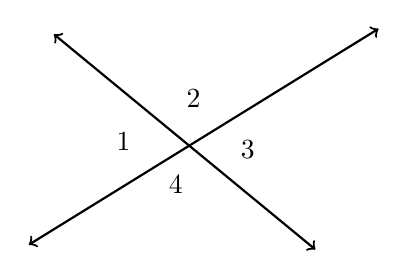
\begin{tikzpicture}[scale=0.5, rotate=15]
    \draw [<->, thick] (0,-1.5)--(10,1.5);
    \draw [<->, thick] (2,3.5)--(7,-3.5);
    \node at (3,.4){1};
    \node at (6,-.6){3};
    \node at (5,1){2};
    \node at (4,-1){4};
  \end{tikzpicture}
  \end{center}
  \end{multicols}

\item Spicy Do Now: A pyramid with a square base has a volume of 576 cubic inches. Its height is the same as the lengths of the sides of the base. Find the area of its base.\\[0.5cm] Given the volume formula $V=\frac{1}{3}(s^2)h$ for a pyramid with a square base ($B=s^2$).
\begin{enumerate}[itemsep=0.5cm]
  \item Write down the variable representing the height
  \item Write down the variable representing the length of the base's side
  \item Write an equation relating the two variables in (a) and (b)
  \item Substitute and solve \[V=\frac{1}{3}(s^2)h\]
\end{enumerate} \vspace{5cm}

\item Given two parallel lines and a transversal, as shown, with $m\angle 6 =  70^\circ$. Write down the value of each angle measure.
  \begin{multicols}{3}
    \begin{enumerate}[itemsep=0.5cm]
      \item $m\angle 1 = $
      \item $m\angle 2 = $
      \item $m\angle 3 = $
      \item $m\angle 4 = $
      \item $m\angle 5 = $
      \item $m\angle 6 = $
      \item $m\angle 7 = $
      \item $m\angle 8 = $
    \end{enumerate}
      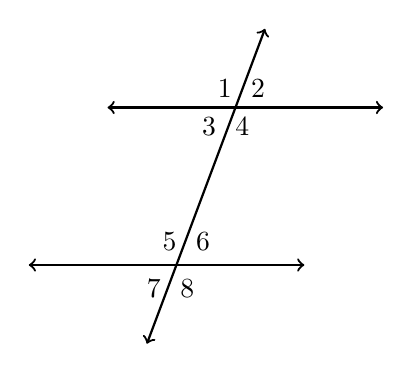
\begin{tikzpicture}[scale=1]
      \draw [<->, thick] (3.5,2)--(7,2);
      \draw [<->, thick] (2.5,0)--(6,0);
      \draw [<->, thick] (4,-1)--(5.5,3);
      \node at (4.5,0.3) [left]{$5$};
      \node at (4.5,0.3) [right]{$6$};
      \node at (4.3,-0.3) [left]{$7$};
      \node at (4.3,-0.3) [right]{$8$};
      \node at (5.2,2) [above left]{$1$};
      \node at (5.2,2) [above right]{$2$};
      \node at (5,2) [below left]{$3$};
      \node at (5,2) [below right]{$4$};
    \end{tikzpicture}
  \end{multicols}

  \newpage
  \item Label the relationship of each pair: adjacent, vertical, corresponding, alternate interior, same side interior, alternate exterior, or same side exterior
  \begin{multicols}{2}
    \begin{enumerate}[itemsep=0.5cm]
      \item $\angle 1$,$\angle 4$
      \item $\angle 3$,$\angle 6$
      \item $\angle 5$,$\angle 3$
      \item $\angle 6$,$\angle 2$
      \item $\angle 1$,$\angle 8$
    \end{enumerate}
      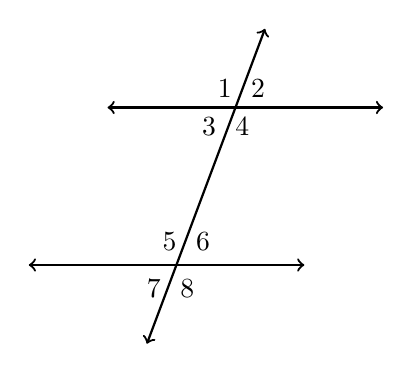
\begin{tikzpicture}[scale=1]
      \draw [<->, thick] (3.5,2)--(7,2);
      \draw [<->, thick] (2.5,0)--(6,0);
      \draw [<->, thick] (4,-1)--(5.5,3);
      \node at (4.5,0.3) [left]{$5$};
      \node at (4.5,0.3) [right]{$6$};
      \node at (4.3,-0.3) [left]{$7$};
      \node at (4.3,-0.3) [right]{$8$};
      \node at (5.2,2) [above left]{$1$};
      \node at (5.2,2) [above right]{$2$};
      \node at (5,2) [below left]{$3$};
      \node at (5,2) [below right]{$4$};
    \end{tikzpicture}
  \end{multicols}

  \item Given two parallel lines and a transversal, with $m\angle 4 = 3x$ and $m\angle 5 = x + 70$. \\ Write an equation, then solve for $x$.
\begin{flushright}
  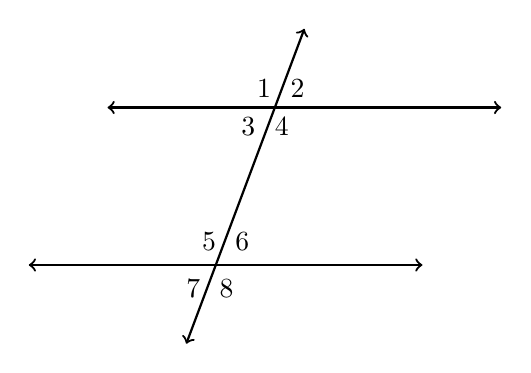
\begin{tikzpicture}[scale=1]
    \draw [<->, thick] (3,2)--(8,2);
    \draw [<->, thick] (2,0)--(7,0);
    \draw [<->, thick] (4,-1)--(5.5,3);
    \node at (4.5,0.3) [left]{$5$};
    \node at (4.5,0.3) [right]{$6$};
    \node at (4.3,-0.3) [left]{$7$};
    \node at (4.3,-0.3) [right]{$8$};
    \node at (5.2,2) [above left]{$1$};
    \node at (5.2,2) [above right]{$2$};
    \node at (5,2) [below left]{$3$};
    \node at (5,2) [below right]{$4$};
  \end{tikzpicture}
\end{flushright} \vspace{2cm}

\item Two parallel lines intersect a transversal. Given corresponding angles  $m\angle 1 = 4.4x - 63$ and $m\angle 2 = 2.8x+9$, find the measure of $\angle 1$. 
  \begin{flushright}
    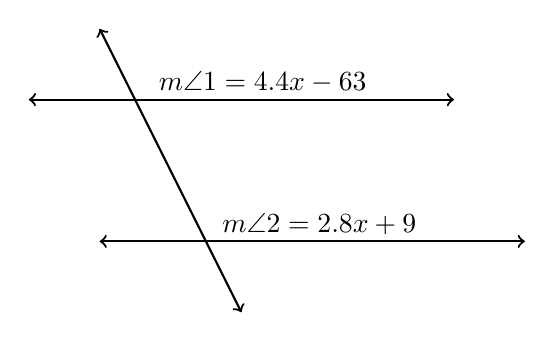
\begin{tikzpicture}[scale=0.9]
      \draw [<->, thick] (3,0)--(9,0);
      \draw [<->, thick] (2,2)--(8,2);
      \draw [<->, thick] (5,-1)--(3,3);
      %\draw [<->, thick] (11,-1)--(9,3);
      %\node at (4, 1.7){$1$};
      \node at (5.3, 2.25){$m\angle 1 = 4.4x - 63$};
      \node at (6.1, 0.25){$m\angle 2 = 2.8x+9$};
      %\node at (10, 0.25){$3$};
    \end{tikzpicture}
    \end{flushright}

\end{enumerate}
\end{document}